\documentclass{article}
\usepackage[colorinlistoftodos]{todonotes}
\usepackage[utf8]{inputenc}
\usepackage{graphicx}

\title{Event propagation through hexagonal indices}
\author{Hernán Carvajal}

\begin{document}

\maketitle

As cities grow in population, they produce large amounts of data, including events from domains like traffic flow, air quality monitoring, crime, epidemic outbreaks, and social media activities. Such spatio-temporal data can help the communities in cities to develop innovative solutions to pressing urban problems\todo{need to add some case examples. Pick one or two examples of why data is important for the develoment of cities}. However, a key challenge is the integration and multi-scale analsysis of different data types collected from varioys sources. Data might represent event at exact locations or an aggregated number of events at different spatial levels of abstraction (granularity) like neighborhoods and municipalities.

To address this problem, it is possible to aggregate the features over the same space within areas such as neighborhoods or postal code zones. One inconvenient with this approach is that such zones might require updating as cities change and often their edges are defined arbitrarily. Moreover, those areas have unusual shapes and sizes, making difficult a direct comparison among them. We used Ubers's H3 hexagonal hierarchical spatial indexing (H3) grid system~\cite{uber2019} to generate spatially continuous hexagons\todo{list the advantages of using hexagons based on the video I sent you}.

An example of visualizing data at different levels is shown in figure~\ref{fig:spatialLevels}. The H3 grid system was originally developed for  data visualization and exploration in the context of pricing optimization for Uber users. Data can be aggregated into hexagonal areas or cells at 16 different resolutions. Additionally, it has an indexing system that allows to group and searches for grouped data efficiently\todo{here say how you extend the exiting framework - by adding a propagatino analysis. then as you have it in the next paragraph finish by specifying you aparticular appliction using tweets and covid data}.

We aggregated geospatial data from different levels to tackle two challenges in the Colombian cities of Bogot\'a and Cali. For the first city, we conduct a study about the impact of the spatio-temporal dynamics of Twitter posts on the sales of a fast-food chain of restaurants; for the second city, we apply the proposed propagation model to better understand the local dynamics of the covid-19 outbreak. In both cases, we took into account demographic variables that are integrated from sources at different scales like the number of inhabitants (available at the block level), percentage of income (neighborhood level), and the presence of places like hospitals, universities, and parks.

\begin{figure}[ptb]
    \centering
    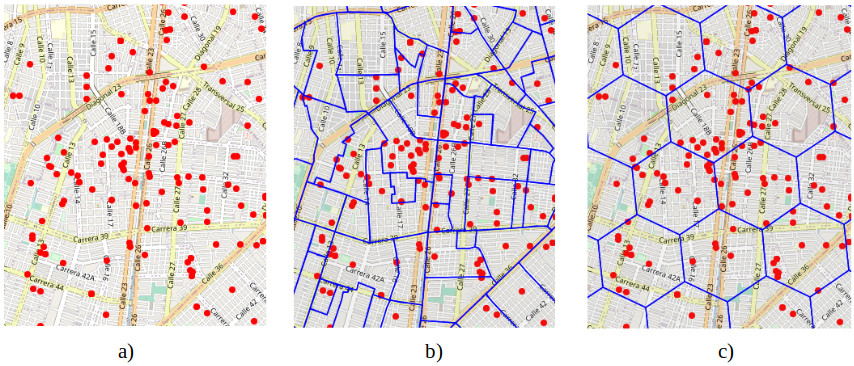
\includegraphics[width=.95\linewidth]{imgs/geolocations}
    \caption{Spatial data at different levels of absraction: a. exact location; b. data grouped by neighborhoods; and c. data grouped by hexagons.}
    \label{fig:spatialLevels}
\end{figure}

\bibliography{bibliografia} 
\bibliographystyle{ieeetr}
\end{document}